\begin{progprob}
    You are given a directed graph representing a tree and a dictionary \python{value}
    which contains a value for each node. Define the \emph{biggest descendent value} of a node $u$ to
    be the largest value of any node which is a descendent of $u$ in the tree (for this problem, you should consider
    $u$ to be a descendent of itself.

    For instance, given the following tree where each node's label is
    replaced by its value:
    \begin{center}
        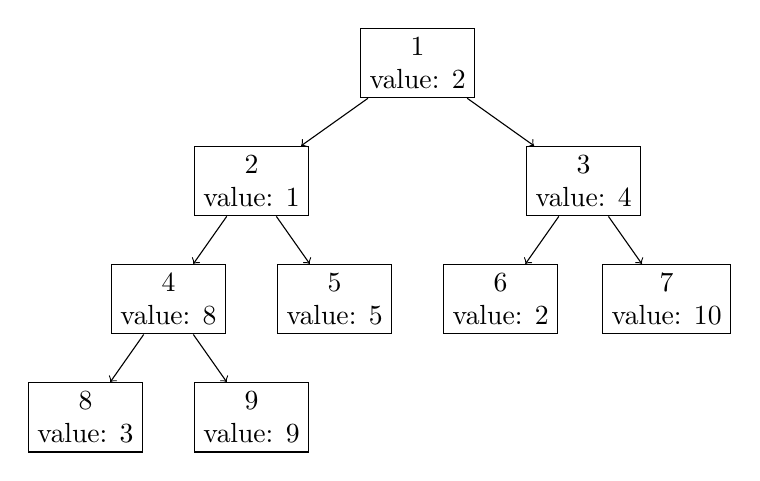
\begin{tikzpicture}[
            level 1/.style={sibling distance=12em},
            level 2/.style={sibling distance=6em},
            every node/.style={align=center, draw},
            ->
            ]
            \node {1\\value: 2}
                child { node {2\\value: 1} 
                    child { node {4\\value: 8} 
                        child { node {8\\value: 3} }
                        child { node {9\\value: 9} }
                    }
                    child { node {5\\value: 5} }
                }
                child { node {3\\value: 4} 
                    child { node {6\\value: 2} }
                    child { node {7\\value: 10} }
                }
                ;
        \end{tikzpicture}
    \end{center}
    The \emph{biggest descendent value} for each node is:
    \begin{center}
        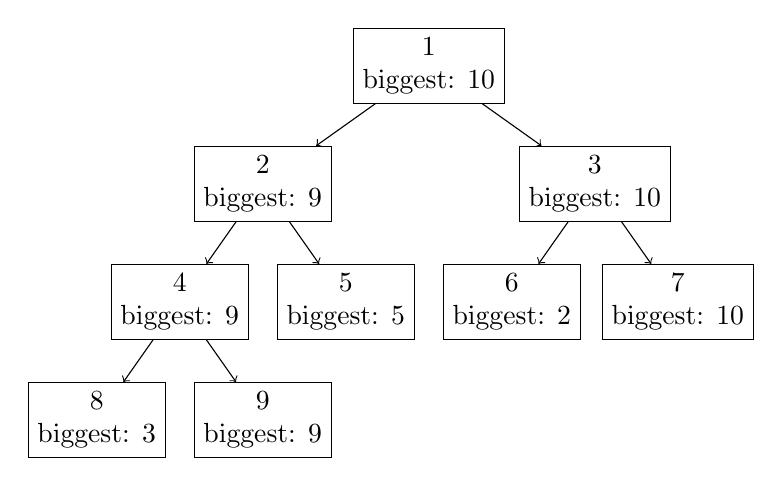
\begin{tikzpicture}[
            level 1/.style={sibling distance=12em},
            level 2/.style={sibling distance=6em},
            every node/.style={align=center, draw},
            ->
            ]
            \node {1\\biggest: 10}
                child { node {2\\biggest: 9} 
                    child { node {4\\biggest: 9} 
                        child { node {8\\biggest: 3} }
                        child { node {9\\biggest: 9} }
                    }
                    child { node {5\\biggest: 5} }
                }
                child { node {3\\biggest: 10} 
                    child { node {6\\biggest: 2} }
                    child { node {7\\biggest: 10} }
                }
                ;
        \end{tikzpicture}
    \end{center}

    In a file named \python{biggest_descendent.py},
    write a function \python{biggest_descendent(graph, root, value)} which accepts
    the graph, the label of the root node, and the dictionary of values and returns
    a dictionary mapping each node in the graph to its biggest descendent value.

    The input graph will be an instance of \python{dsc40graph.DirectedGraph()}.

    Example:

    \begin{minted}[autogobble]{python}
        >>> edges = [(1, 2), (1, 3), (2, 4), (2, 5), (4, 8), (4, 9), (3, 6), (3, 7)]
        >>> g = dsc40graph.DirectedGraph()
        >>> for edge in edges: g.add_edge(*edge)
        >>> value = {1: 2, 2: 1, 3: 4, 4: 8, 5: 5, 6: 2, 7: 10, 8:3, 9: 9}
        >>> biggest_descendent(g, 1, value)
        {1: 10, 2: 9, 3: 10:, 4: 9, 5: 5, 6: 2, 7: 10, 8: 3, 9: 9}
    \end{minted}

    \begin{soln}
        % write your solution here
    \end{soln}
\end{progprob}
